%% ===========================================================
%%  Constraint Satisfaction in Time-Series Foundation Models
%%  Neurocomputing submission format (single-anonymized review, so the
%%  author details are in the front matter below). Reference style:
%%  numbered, in order of appearance (elsarticle-num).
%%  Compile: pdflatex main && bibtex main && pdflatex main && pdflatex main
%%  Highlights are in the SEPARATE file highlights.txt.
%% ===========================================================
%% `review` = double-spaced + line numbers, convenient for referees.
%% For comfortable reading, change `review` to `preprint` (single-spaced).
\documentclass[review,number]{elsarticle}

\usepackage[T1]{fontenc}   % accented author names as single glyphs (searchable, copyable)
\usepackage{lmodern}       % scalable Type 1 fonts; T1 alone would pull bitmap fonts
\usepackage{lineno}
\usepackage{amsmath,amssymb}
\usepackage{booktabs}
\usepackage{graphicx}
\usepackage[hidelinks]{hyperref}
\usepackage{xcolor}

%% Floats may also sit at the bottom of a page or on a float page, and may fill
%% most of a page; with the class defaults a tall table that is restricted to the
%% top of a page can never be placed and drags every later float to the end.
\renewcommand{\topfraction}{0.95}
\renewcommand{\bottomfraction}{0.7}
\renewcommand{\textfraction}{0.05}
\renewcommand{\floatpagefraction}{0.8}

%% Allow a little extra stretch so long monospace identifiers and the mandated
%% (very long) generative-AI section heading do not overrun the text block.
\emergencystretch=3em
\hyphenation{datasets-forecast hierarchical-forecast}

\journal{Neurocomputing}

%% Suppress the class's "Preprint submitted to ... <date>" footer on page one.
\makeatletter
\def\ps@pprintTitle{%
  \let\@oddhead\@empty \let\@evenhead\@empty
  \let\@oddfoot\@empty \let\@evenfoot\@oddfoot}
\makeatother

\begin{document}

\begin{frontmatter}

\title{Constraint Satisfaction in Time-Series Foundation Models:
A Multi-Model Audit of Coherence Failures}

\author[uah]{Lino González García}
\ead{lino.gonzalez@uah.es}
\author[uah]{Loukas Samaras}
\ead{lsamaras@ath.forthnet.gr}
\author[uah]{Elena García-Barriocanal}
\ead{elena.garciab@uah.es}
\author[uah]{Miguel-Angel Sicilia\corref{cor1}}
\ead{msicilia@uah.es}
\cortext[cor1]{Corresponding author.}
\affiliation[uah]{organization={Computer Science Department, Escuela Politécnica
  Superior, University of Alcalá},
  addressline={Campus Universitario, Ctra. Madrid-Barcelona Km.\ 33.600},
  postcode={28805},
  city={Alcalá de Henares, Madrid},
  country={Spain}}

\begin{abstract}
Time-series foundation models produce forecasts for each series, and nothing in them
constrains the forecasts for the parts of a hierarchy to sum to that for the whole, a
property called coherence. How often this linear coupling is violated, whether the rate
depends on the model, and what it costs to remove it on a model that cannot be refitted
have not been measured. We audit six foundation models on eight hierarchies and compare
bottom-up, trace-minimisation and learned reconciliation on point and probabilistic
forecasts. On six of the eight hierarchies most aggregate forecasts are incoherent for
every foundation model but the least accurate, at rates that do not vary with model size
or accuracy. Joint forecasting narrows the gaps without closing them, and a single series
forecast at monthly and annual scale contradicts itself on up to four fifths of its
aggregates. On a frozen base the learned reconcilers are unstable, because the base
affords few in-sample origins, and bottom-up reconciliation is the reliable choice, at a
small cost in accuracy; across time scales it improves accuracy. For predictive
distributions the cost of summing independent marginals does not grow with cross-series
dependence, whereas coupling the series with a copula lowers it most where dependence is
strongest. Accuracy varies more among foundation models than between them and a
classical model, so it does not identify a base. A forecasting system should therefore
project whichever base is most accurate onto its constraints; an ablation shows that the
projection step alone supplies the guarantee.
\end{abstract}

\begin{keyword}
Time-series foundation models \sep Constraint satisfaction \sep Hierarchical coherence
\sep Temporal aggregation \sep Probabilistic forecast reconciliation \sep Forecast evaluation
\end{keyword}

\end{frontmatter}

\linenumbers

% ============================================================
\section{Introduction}
\label{sec:intro}
Time-series forecasting has seen the rapid appearance of \emph{foundation models}:
pretrained networks such as Chronos~\citep{chronos2024},
Chronos-2~\citep{chronos2_2025}, TimesFM~\citep{timesfm2024}, Moirai~\citep{moirai2024}
and
Lag-Llama~\citep{lagllama2024}, which produce zero-shot forecasts without per-series
modelling. Benchmarks such as GIFT-Eval~\citep{gifteval2024} and
fev-bench~\citep{fevbench2025} report models of this kind matching or outperforming
automatic statistical baselines in aggregate, though not in every regime.

Those benchmarks do not measure whether the forecasts satisfy the constraints that
couple them. A model that forecasts each
series independently cannot satisfy a \emph{linear coupling} constraint, however
accurate each individual forecast is. The most familiar case is hierarchical
coherence: the forecasts for a country's regions must sum to the forecast for the
country~\citep{mint2019,hfreview2024}. The same holds for any cross-series
accounting identity. The constraint need not involve a second series. A
monthly series is coupled to its own annual aggregate, so a model queried at both scales
must agree with itself. Independent forecasting fails in both cases for the same reason,
that nothing in the model constrains the outputs it produces separately. Per-series
modelling is one way of
lacking such a constraint, and a model trained jointly across the whole hierarchy is
equally free to violate it; we confirm that two trained global models do, at rates
comparable to the per-series ones. Per-series zero-shot forecasting is the clearest case of
that failure. The agentic forecasting systems recently proposed do not supply a
constraint either~\citep{tsci2025,nexus2026,dcats2025}. They organise selection,
reasoning and data curation around a forecaster, or have a language model produce the
forecast directly, and do not constrain the forecasts they emit.
Coherence is therefore violated by construction, regardless of model quality, and is
restored only by an explicit reconciliation or assembly step.

Two further results, on accuracy and on non-negativity, bound this one. The first
concerns accuracy, the property that benchmarks measure. Foundation-model accuracy is
heterogeneous. On the same data a
ten-parameter classical model outperforms one widely used foundation model at every
history length on the smooth data yet is less accurate than another at most of
them. Per-series Diebold--Mariano tests cannot separate it
from them on about $81\%$ of smooth series. The axis along which these models are
ranked therefore discriminates weakly at the level where forecasts are used, and no
conclusion drawn from a single foundation model transfers to the others. Few benchmarks
vary the per-series history length. Concurrent work that varies the training
size of the classical models~\citep{breakeven2026} or the context
length~\citep{quitobench2026,energyload2026} also finds that the verdict between
foundation models and smaller ones changes along it, but none of it connects the
finding to coherence. The second result bounds the
coherence claim. Per-series constraints such as non-negativity are satisfied by
one foundation model (through a positivity safeguard in its inference library) and violated without
warning by the rest. Constraint satisfaction is thus not uniformly absent, and the
coupling failure is not general inattention to constraints.

We make four contributions.

First, we show that coherence is violated by every foundation model we test, each run
per series, across the series of a hierarchy and across the time aggregations of a single
series. The rates are independent of accuracy and of model size. Point reconciliation
removes the violation exactly, and in the temporal case bottom-up aggregation also
improves accuracy. On a frozen base, however, the reconcilers that estimate a weight
matrix are unstable, because such a base affords few in-sample origins, and bottom-up
is the reliable choice; this reverses the usual recommendation for fitted base
forecasters.

Second, we show that probabilistic coherence is more demanding. Summing independent marginals is
inexpensive on most hierarchies and does not scale with cross-series dependence,
contrary to what a smaller sample had suggested. Copula coupling lowers the cost further, most where
dependence is strongest, because per-series models supply no joint distribution.
An accurate coherent predictive distribution therefore remains open.

Third, we provide a multi-model audit covering six foundation models, two trained global
baselines, eight hierarchies and a per-series history-length frontier. On six of the
eight hierarchies coherence is violated by every model we evaluate, whether the
base is zero-shot or globally trained, while accuracy and non-negativity are
model-dependent.

Fourth, we introduce \emph{constraint-aware assembly} (CAA). CAA projects a small
interpretable base onto the declared feasible set by reconciliation, clipping or isotonic
projection, so its forecasts are coherent and feasible by construction. An ablation shows
that the feasibility comes from the projection step; conditioning the model selection
on the constraints does not change it.

CAA is a forecasting system rather than a new reconciliation method. It reads a
declared constraint specification, selects a model from a small interpretable library
by data-derived features, and then enforces feasibility by projecting onto the declared
constraint set (reconciliation, clipping, isotonic projection). The projection is the
step that provides the guarantee. Bottom-up and trace-minimization reconciliation are
standard~\citep{mint2019,hfreview2024}, and CAA adds no reconciliation operator. Its
contribution is the packaging of automated feasibility enforcement into a small,
interpretable system, together with the systematic evidence that foundation models
require it.

% ============================================================
\section{Related work}
\label{sec:related}
Five lines of work bear on this paper. The first two concern how foundation models are
currently evaluated. We take their findings as established and draw methodological
choices from them. The last three concern constraint satisfaction,
and the coherence contribution is positioned against them.

\paragraph{Simple-baseline critiques} DLinear~\citep{dlinear2023} showed linear
projections rival transformers, and \citet{toner2024linear} showed that popular linear
forecasters reduce to closed-form regression. \citet{benchmarking2026} make the
complementary methodological argument that current benchmarking practice does not
isolate which design choices produce the differences it reports. We take this line of
evidence as established and do not revisit it. It is the reason we accompany
aggregate accuracy with significance tests, including per-series ones
(Section~\ref{sec:frontier}).

\paragraph{Cost frontiers and the history axis} The cost-versus-accuracy axis has
been studied by \citet{operationalviability2026}, who route each series to a model
class using empirically derived features and report a large inference-cost saving under
their cost model. The history axis has been varied in three ways that should not be
conflated. \citet{energyload2026} evaluate on consumer hardware while sweeping the
history window from $24$ to $2048$ steps, which is the context of the foundation models
and the fitting window of the classical baselines, the design closest to ours.
\citet{breakeven2026} vary the training fraction of the classical models from $2\%$ to
$100\%$, the foundation models always receiving the full history, and report a
break-even sample size. \citet{quitobench2026} report a crossover along context length
between trained deep-learning models and foundation models. Separately,
\citet{foundational2025} show a small model trained from scratch outperforming a
fine-tuned foundation model on a domain-specific electricity series. In all of this
work the verdict between foundation models and smaller ones changes with data size,
context or domain on some datasets and not on others, and one applied
study under data scarcity finds it to depend on the series and the model
family~\citep{enrolment2026}. None of this work connects the finding to
coherence.

\paragraph{Agentic selection} TimeSeriesScientist~\citep{tsci2025} diagnoses,
selects and ensembles models from a fixed library of statistical, machine-learning and
neural forecasters. Nexus~\citep{nexus2026} decomposes forecasting
into reasoning stages that fold in textual context, and DCATS~\citep{dcats2025} uses
metadata to curate the training data rather than to choose a model. In a position paper
on the paradigm, \citet{atsf2026} list human-supplied preferences, constraints and domain
knowledge among its opportunities, as inputs to planning and evaluation rather than as
restrictions on the forecasts. None of
the systems we surveyed enforces hard constraints on the forecasts it emits.

\paragraph{Forecast reconciliation} Reconciling incoherent forecasts onto a
hierarchy is a mature literature: bottom-up and top-down schemes, the
trace-minimization optimum MinT~\citep{mint2019}, and the probabilistic extension with
its scoring-rule evaluation~\citep{probrecon2023}, surveyed, temporal hierarchies
included, by \citet{hfreview2024}. We
apply these methods and do not extend them. The new element is the base forecaster to
which they are applied. That literature accepts base forecasts from any source, although the reconcilers
that estimate a covariance or weight matrix need in-sample forecast errors,
traditionally the residuals of models the analyst fits, and it asks which
reconciliation is optimal. We instead ask how much
reconciliation a frozen zero-shot model needs, whether the need varies with its
accuracy or size, and what it costs. These questions only arise once the base
forecaster is one the analyst cannot refit.

\paragraph{Constrained models} ProbHardE2E~\citep{probharde2e2025} enforces hard
constraints through a differentiable projection layer trained end-to-end, and argues
that imposing constraints only as a post-processing step, rather than also during
training, forgoes an end-to-end solution;
\citet{doumeche2025} give a unified treatment of linear constraints, hierarchical
forecasting among them, imposed during training and solvable by linear algebra alone;
Auto-PINN~\citep{autopinn2022} searches architectures for physics-informed networks that
solve differential equations. Each of these
requires control of the model being trained. A foundation model is used frozen and
zero-shot, so a constraint can only be imposed on
its output. We therefore forgo the end-to-end training whose accuracy benefit
\citet{probharde2e2025} report, in exchange for a step that applies to any base
forecaster, and we measure what that costs. For point reconciliation the cost is small
(Section~\ref{sec:coherence}); for predictive distributions it is the subject of
Section~\ref{sec:probcoh}.

None of these lines covers the setting of this paper. Reconciliation has been studied
on base forecasters that the analyst fits, and constrained training assumes a model that
the analyst trains; benchmarks and agentic systems do not raise the question. A frozen
zero-shot base, chosen from several whose coherence behaviour has not, to our knowledge,
been measured,
falls outside all three. This paper audits that setting, and constraint-aware
assembly is built for it (Table~\ref{tab:gap}).

\begin{table}[tbp]
\centering
\small
\begin{tabular}{lccc}
\toprule
& Coherent by & Multi-model & Feasibility \\
& construction & coherence audit & enforced \\
\midrule
Foundation models                   & $\times$ & $\times$ & $\times$ \\
fev-bench / GIFT-Eval               & $\times$ & $\times$ & $\times$ \\
Cost-frontier studies               & $\times$ & $\times$ & $\times$ \\
Agentic forecasters                 & $\times$ & $\times$ & $\times$ \\
Reconciliation methods              & \checkmark & $\times$ & single-base \\
CAA (this paper)                   & \checkmark & \checkmark & \checkmark \\
\bottomrule
\end{tabular}
\caption{Existing work studies base forecasters that the analyst fits or trains. To our
knowledge, no work audits a frozen zero-shot base across models and returns it feasible
by construction.}
\label{tab:gap}
\end{table}

% ============================================================
\section{Methodology}
\label{sec:methodology}

\subsection{Problem formulation}
\label{sec:formulation}
Let $y_{1:T}$ be a series with history length $T$ and horizon $h$. A constraint
set $\mathcal{C}$ collects declared restrictions on admissible forecasts
$\hat{y}_{T+1:T+h}$: non-negativity $\hat{y}_t \ge 0$; capacity $\hat{y}_t \le c$;
monotonicity $\hat{y}_{t+1} \ge \hat{y}_t$; or hierarchical coherence
$S\hat{y}_{\text{bottom}} = \hat{y}_{\text{all}}$ for a summing matrix
$S$~\citep{mint2019}. We evaluate forecasters on two axes: accuracy (mean absolute scaled
error, MASE) and constraint satisfaction
(the fraction of forecast points or nodes that violate $\mathcal{C}$). The assembled
forecaster is additionally
interpretable by construction, having few parameters, closed-form fitting and
an emitted rationale, though we treat this as a design property and do not benchmark
it.

\subsection{Constraints audited}
\label{sec:whichconstraints}
The restrictions collected in
$\mathcal{C}$ fall into two classes, and that division is itself the object of study.
\emph{Coupling} constraints bind several series simultaneously (hierarchical
coherence, accounting identities, no-arbitrage relations, conservation laws), and a
forecaster that maps each series independently cannot satisfy them at all, however
accurate it is. \emph{Within-series} constraints bind each series on its
own (non-negativity, capacity, monotonicity), and a per-series forecaster can
satisfy them perfectly well; whether it does is a matter of implementation. We audit
two exemplars of the coupling class, coherence across series and
coherence across time aggregations of a single series, and one exemplar of the
within-series class, instead of surveying many, because the contrast between
the classes identifies the failure as structural. If every constraint were violated,
the only available conclusion
would be that these models disregard declared constraints indiscriminately. One
constraint is satisfied exactly by one model (Section~\ref{sec:nonneg}), and another is
satisfied by no model, not even a ten-parameter classical one
(Section~\ref{sec:coherence}). The contrast shows which constraints a per-series
forecaster is unable to satisfy.

Within those classes the exemplars are chosen for measurability. Hierarchical
coherence is the best-instrumented coupling constraint. It has a canonical linear
formalization through $S$, public benchmark hierarchies and an established
reconciliation literature against which the correction can be judged. Other coupling
constraints, such as no-arbitrage or physical conservation, have no comparable public
benchmarks.
Temporal coherence is included as a second coupling exemplar because it
requires no second series. This removes the objection that a hierarchy should
have been modelled jointly (Section~\ref{sec:temporal}).
Non-negativity is the cleanest within-series constraint. Its ground truth is
unambiguous, and it binds on intermittent demand, where forecasts lie
against the boundary. Capacity and monotonicity are stated above to show
the generality of the formulation; capacity is used in the ablation of
Section~\ref{sec:frontier}, but neither is audited separately, because realistic
ceilings and monotone regimes are not supplied with public benchmark data and would
have to be imposed synthetically. Such evidence is weaker than that of a constraint that
holds in the data by construction.

For the accuracy axis we hold the test window fixed and sweep the available history
$T$ per series, an axis that standard foundation-model benchmarks do not vary as an
experimental factor and that only recent concurrent work has begun to vary. The crossover between a small
model and a foundation model need not exist, and we find that its location depends on
which foundation model is used.

\subsection{Constraint-aware assembly}
\label{sec:caa}
CAA proceeds in four stages: (1) \emph{diagnose} statistical features of $y_{1:T}$
(trend, seasonal strength, intermittency, length); (2) \emph{read} the declared
constraint set $\mathcal{C}$; (3) \emph{assemble} a small model from an
interpretable library (seasonal naive, Theta, ETS, ARIMA, and Croston for intermittent
demand); and (4) \emph{project} the
raw forecast onto the feasible set induced by $\mathcal{C}$ (clipping, isotonic
projection or reconciliation) and emit a natural-language rationale. The output is
guaranteed feasible. This guarantee distinguishes CAA from
the agentic systems surveyed above, none of which enforces hard constraints, and it
comes from the projection step. An ablation (Section~\ref{sec:frontier}) that
also conditions the selection in stage~(3) on the declared constraints finds that it
changes the chosen base on $27\%$ of series yet does not change accuracy
(paired $p=0.97$), while feasibility is achieved by projection in either case. We
therefore present CAA as constraint-aware projection of a selected
interpretable base, and do not claim constraint-conditioned selection as a benefit.

\subsection{Experimental design}
\label{sec:design}
We evaluate six foundation models zero-shot on the GPU: TinyTimeMixer~\citep{ttm2024};
Chronos-Bolt and Chronos-Bolt-Base, later releases of Chronos~\citep{chronos2024} by its
authors that the cited paper does not itself describe; Chronos-2~\citep{chronos2_2025};
Moirai~\citep{moirai2024}, in its 1.1-R small release; and TimesFM~2.5, a later release
of the model introduced by \citet{timesfm2024}. We compare them
against a small statistical library
(AutoARIMA, AutoETS, AutoTheta, Croston, seasonal naive) from which CAA assembles. To
test whether the coherence failure is specific to per-series or zero-shot forecasting, we
add two \emph{trained global} baselines, a gradient-boosted LightGBM over lagged and
rolling features and a dilated causal-convolution TCN, each fit jointly across all
series of a hierarchy. Chronos-2 and Moirai also accept covariates and can forecast
several series jointly~\citep{chronos2_2025,moirai2024}. We run every model in
univariate mode, one node per call, on integer-indexed hierarchies
without exogenous covariates, so the eight hierarchies are directly comparable. Neither
paper describes a summing constraint on the joint outputs. We test Chronos-2's joint
mode separately, passing all nodes of a hierarchy as the variates of one task
(Section~\ref{sec:coherence}), and
return to covariates and joint forecasting in Section~\ref{sec:discussion}.
TinyTimeMixer enters the coherence audits only. It emits point forecasts without
predictive quantiles, so it is excluded from the probabilistic study instead of being
assigned a degenerate distribution. The remaining experiments use the five models
that supply quantiles. Three experimental settings isolate the reported findings.
Table~\ref{tab:datasets} lists every dataset they use, with its size, forecast horizon,
number of rolling origins and the study it serves.

% AUTO-GENERATED by tsfm_bench.tables. Do not edit by hand.
\begin{table}[tbp]
\centering
\footnotesize
\setlength{\tabcolsep}{3pt}
\begin{tabular}{llrrrrrrl}
\toprule
Dataset & Freq. & Series & Bottom & Aggr. & $h$ & Origins & $\bar\rho$ & Section \\
\midrule
Wiki2 & daily & 199 & 150 & 49 & 14 & 8 & 0.04 & \ref{sec:coherence}--\ref{sec:probcoh} \\
TourismLarge & monthly & 555 & 304 & 251 & 12 & 8 & 0.11 & \ref{sec:coherence}--\ref{sec:probcoh} \\
Labour & monthly & 57 & 32 & 25 & 8 & 8 & 0.19 & \ref{sec:coherence}--\ref{sec:probcoh} \\
TourismSmall & quarterly & 89 & 56 & 33 & 4 & 7 & 0.31 & \ref{sec:coherence}--\ref{sec:probcoh} \\
M5 retail & daily & 84 & 70 & 14 & 28 & 8 & 0.34 & \ref{sec:coherence}--\ref{sec:probcoh} \\
Traffic & daily & 207 & 200 & 7 & 14 & 8 & 0.44 & \ref{sec:coherence}--\ref{sec:probcoh} \\
Electricity & hourly & 46 & 40 & 6 & 24 & 8 & 0.63 & \ref{sec:coherence}--\ref{sec:probcoh} \\
Solar & hourly & 152 & 137 & 15 & 24 & 8 & 0.70 & \ref{sec:coherence}--\ref{sec:probcoh} \\
\midrule
M4 monthly & monthly & 481 & --- & --- & 18 & 8 & --- & \ref{sec:frontier} \\
M4 quarterly & quarterly & 536 & --- & --- & 8 & 8 & --- & \ref{sec:frontier} \\
M5 daily & daily & 995 & --- & --- & 14 & 8 & --- & \ref{sec:frontier} \\
M4 monthly & monthly & 400 & --- & --- & 12 & 4 & --- & \ref{sec:temporal} \\
M3 monthly & monthly & 1200 & --- & --- & 12 & 1 & --- & \ref{sec:nonneg} \\
M5 daily & daily & 1197 & --- & --- & 28 & 1 & --- & \ref{sec:nonneg} \\
M4 monthly (capacity) & monthly & 300 & --- & --- & 18 & 1 & --- & \ref{sec:frontier} \\
\bottomrule
\end{tabular}
\caption{Datasets used in each study. For the eight hierarchies (top), Series is the number of nodes, split into bottom and aggregate nodes; $h$ is the forecast horizon, Origins the number of rolling origins, and $\bar\rho$ the cross-series dependence (mean $|$correlation$|$ of the bottom series' first differences). The non-hierarchical datasets (bottom) are listed once per study with the number of series that study used.}
\label{tab:datasets}
\end{table}


\paragraph{Coherence (Sections~\ref{sec:coherence}--\ref{sec:probcoh})} On eight real
hierarchies we forecast every node independently and measure the fraction of aggregate
nodes whose forecasts differ from the sum of their children by more than $1\%$. Five are
the benchmark hierarchies distributed with the \texttt{datasetsforecast}
package~\citep{datasetsforecast}: the Australian domestic-tourism hierarchies
TourismSmall ($89$ series) and TourismLarge ($555$ series) of \citet{hyndman2011} and
\citet{mint2019}, built from Tourism Research Australia's National Visitor
Survey~\citep{data_tourism}; Labour, Australian labour-force series grouped by region,
gender and employment status; and the Traffic and Wiki2 hierarchies of
\citet{bentaieb2019erm}. The sixth is a retail
hierarchy we construct from M5~\citep{data_m5} (Total $\to$ state $\to$ store $\to$
store\,$\times$\,department; $70$ bottom series, $14$ aggregates). Because these span
little of the upper cross-series dependence axis, we add two high-dependence energy
hierarchies built the same way (summing matrix $S$ verified so that
$\max|S y_{\text{bottom}}-y_{\text{all}}|=0$ on the data): \emph{Solar} ($137$ PV stations
grouped Total $\to$ group $\to$ station, $15$ aggregates, mean bottom-series correlation
$0.70$) and \emph{Electricity} ($40$ consumption feeders grouped Total $\to$ group $\to$
feeder, $6$ aggregates, correlation $0.63$). Both are built from the hourly multivariate
collections used by \citet{salinas2019gpcopula} and distributed with
GluonTS~\citep{gluonts2020} as \texttt{solar\_nips} ($137$ series) and
\texttt{electricity\_nips} ($370$ Portuguese consumption series, originally
\citet{data_electricity}), whose clients we group into $40$ feeders because the raw
clients are only moderately dependent ($0.27$) and would not populate the high end we
need. We then reconcile each base forecast
(bottom-up; MinTrace in its OLS and shrinkage forms; and the learned ERM reconciler of
\citet{bentaieb2019erm}) and
report the accuracy of the coherent point forecasts, as the mean scaled error over every
node of the hierarchy, bottom and aggregate alike. For probabilistic coherence we
draw samples from each
node's predictive quantiles, reconcile bottom-up in sample space by summing
independent marginals and after two couplings that impose historical cross-series
dependence, a Schaake shuffle~\citep{schaake2004} on historical observations and a
fitted Gaussian copula, and score with CRPS over up to eight rolling origins. On the
most recent origin of each hierarchy we also record the wall-clock time of every step,
from inference to coupling. Times are measured on one NVIDIA GB10 system (Grace
Blackwell, 20 Arm cores, 128~GB of unified memory), with inference on its GPU and
reconciliation on its CPU.

\paragraph{Non-negativity (Section~\ref{sec:nonneg})} On strictly non-negative series,
M3~\citep{data_m3} (values far from zero) and M5 retail~\citep{data_m5} (intermittent
counts near zero), we measure how often each foundation model's median and lower
predictive band fall below zero.

\paragraph{Accuracy versus history (Section~\ref{sec:frontier})} On M4 monthly and
quarterly~\citep{data_m4} and M5 daily we hold the test window fixed and truncate the
available history $T$ on a grid matched to each frequency, $\{12,24,48,96,192,384\}$
months, $\{8,16,32,64,128\}$ quarters and $\{28,56,112,224\}$ days; only the input
history changes.
We report mean MASE against $T$ with eight rolling origins, $95\%$ bootstrap
confidence intervals, and win-rates against each foundation model.

% ============================================================
\section{Results}
\label{sec:results}

\subsection{Incoherence across models and hierarchies}
\label{sec:coherence}
We forecast each node of eight real hierarchies independently with six foundation
models (TinyTimeMixer, Chronos-Bolt, Chronos-Bolt-Base, Chronos-2, Moirai and TimesFM),
a small statistical model (AutoETS), and two trained global models that forecast every
node jointly (a LightGBM and a dilated-convolution TCN, both fit across all series of
the hierarchy). The global models test whether the failure is specific to per-series
forecasting. We measure the share of aggregate nodes whose forecasts do not equal the
sum of their children (relative gap above $1\%$). Table~\ref{tab:coherence} shows that on
six of the eight hierarchies the great majority of aggregate nodes are incoherent, at
$68.8$--$100\%$ for every foundation model on those six, TinyTimeMixer aside. This
includes Chronos-2, the most recently released of the models tested and, on several
hierarchies, the most accurate.
The two exceptions, Labour and Electricity, are the hierarchies whose
aggregates consist mostly of a common smooth component, which the independent forecasts
reproduce almost exactly. In neither case does a model enforce the constraint.

Because a count depends on the tolerance, we also report the size of the gaps behind it.
Averaged over the foundation models, the typical relative gap at an aggregate node is
$11.6\%$ on Wiki2 and $13.5\%$ on TourismLarge, and $4.2$--$4.9\%$ on TourismSmall,
Traffic and Solar. On those five the typical gap is four to thirteen times the $1\%$
tolerance, so the counts do not depend on where it is drawn. M5 retail is the
exception among the affected hierarchies, at $1.7\%$. There the mismatches lie close to
the tolerance, and a looser tolerance would lower the count. On Labour ($0.6\%$) and
Electricity ($0.8\%$) the typical gap falls below the tolerance altogether. This
measures directly the common smooth component that the counts had only suggested.

The set of models deliberately spans two orders of magnitude of capacity, from the
$0.8$M-parameter TinyTimeMixer checkpoint to the roughly $200$M-parameter TimesFM and
Chronos-Bolt-Base, and incoherence does
not vary with that scale. On the six affected hierarchies the foundation models are
incoherent at indistinguishable rates regardless of size. TinyTimeMixer supplies the
only low values on those hierarchies (M5 retail $21\%$, Solar $28\%$), but these do not
indicate better behaviour, because TinyTimeMixer is also the least accurate of the six
foundation models on seven of the eight hierarchies (Moirai is less accurate on
Electricity). A sufficiently flat forecast is closer to
coherent without being useful. Incoherence is therefore independent of capacity as well
as of accuracy. The small AutoETS model is incoherent at comparable rates
to the foundation models, and so are the two trained global models. LightGBM is
incoherent on $50$--$100\%$ of aggregate nodes and the TCN on $21$--$100\%$, although
both are fit jointly across the whole hierarchy. Incoherence is thus a property of any
forecaster that does not constrain its outputs to the coupling set, and forecasting
each series independently is only the clearest case of it. Accuracy and joint training
do not remove it (Figure~\ref{fig:coherence}).

Chronos-2 allows the joint-modelling objection to be tested on a foundation model
directly, because it can forecast all nodes of a hierarchy as the variates of one task
and share information across them. Run this way it remains incoherent, on $3$--$100\%$
of aggregate nodes across the eight hierarchies. On five of the six affected hierarchies
the majority of aggregates still fail (TourismSmall $69\%$, TourismLarge $89\%$, Traffic
$95\%$, Wiki2 $99\%$, Solar $100\%$), and on M5 retail the share falls from $74\%$ to
$31\%$. Joint forecasting does narrow the gaps. The typical relative gap falls on seven
of the eight hierarchies (Traffic $3.9\% \to 1.8\%$), and accuracy improves on two
(Traffic $1.267 \to 1.115$ MASE, TourismSmall $0.956 \to 0.869$) and stays within $0.02$
elsewhere. Sharing information across series therefore reduces incoherence without
removing it, since it is not a constraint on their sum.

\begin{figure}[tbp]
\centering
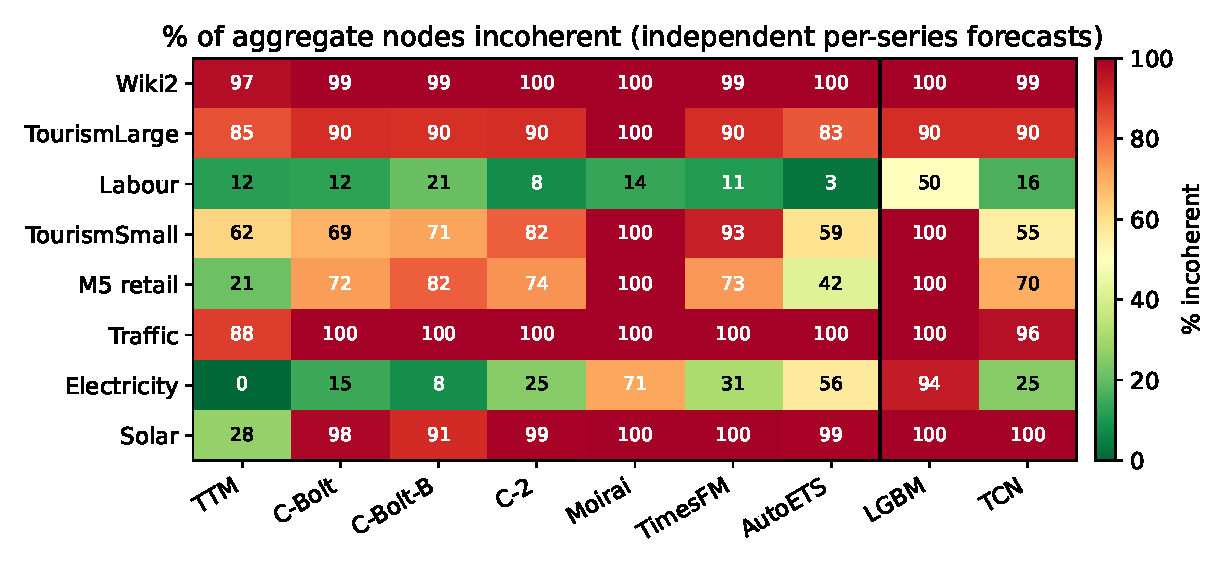
\includegraphics[width=\linewidth]{figures/coherence_incoherence.pdf}
\caption{Percentage of aggregate nodes with incoherent forecasts, by hierarchy (in
ascending cross-series dependence) and model. The two trained global models
(LightGBM, TCN) are to the right of the rule.}
\label{fig:coherence}
\end{figure}

% AUTO-GENERATED by tsfm_bench.tables. Do not edit by hand.
\begin{table}[tbp]
\centering
\footnotesize
\setlength{\tabcolsep}{2pt}
\resizebox{\linewidth}{!}{%
\begin{tabular}{lrrrrrrrrr}
\toprule
\multicolumn{1}{c}{} & \multicolumn{6}{c}{foundation (zero-shot)} & \multicolumn{1}{c}{classical} & \multicolumn{2}{c}{trained global} \\
Hierarchy (agg.) & TTM & C-Bolt & C-Bolt-B & C-2 & Moirai & TimesFM & AutoETS & LGBM & TCN \\
\midrule
Wiki2 ($49$) & 96.7 & 99.5 & 99.5 & 99.7 & 100.0 & 99.5 & 100.0 & 100.0 & 99.0 \\
TourismLarge ($251$) & 84.6 & 90.3 & 90.2 & 90.3 & 100.0 & 90.2 & 83.3 & 90.4 & 90.4 \\
Labour ($25$) & 12.0 & 12.5 & 21.0 & 8.0 & 14.0 & 11.0 & 3.0 & 50.0 & 21.0 \\
TourismSmall ($33$) & 62.3 & 68.8 & 71.4 & 82.3 & 99.6 & 93.1 & 58.9 & 100.0 & 55.4 \\
M5 retail ($14$) & 21.4 & 72.3 & 82.1 & 74.1 & 100.0 & 73.2 & 42.0 & 100.0 & 71.4 \\
Traffic ($7$) & 87.5 & 100.0 & 100.0 & 100.0 & 100.0 & 100.0 & 100.0 & 100.0 & 100.0 \\
Electricity ($6$) & 0.0 & 14.6 & 8.3 & 25.0 & 70.8 & 31.2 & 56.2 & 93.8 & 20.8 \\
Solar ($15$) & 27.5 & 98.3 & 90.8 & 99.2 & 100.0 & 100.0 & 99.2 & 100.0 & 100.0 \\
\bottomrule
\end{tabular}
}
\caption{Percentage of aggregate nodes that are incoherent (relative gap between the forecast and the sum of its children above $1\%$), averaged over up to eight rolling origins; the number of aggregate nodes is in parentheses. Bottom-up reconciliation drives every entry to zero. TTM = TinyTimeMixer; C-Bolt = Chronos-Bolt; C-Bolt-B = Chronos-Bolt-Base; C-2 = Chronos-2; LGBM = LightGBM.}
\label{tab:coherence}
\end{table}


The remedy is an explicit reconciliation or assembly step. Bottom-up reconciliation
attains coherence by construction. It discards the model's own forecast at each
aggregate node and replaces it with the sum of that node's children, after which the two
cannot disagree. Coherence therefore holds by definition, and the open question is its
cost in accuracy. The cost is small (Table~\ref{tab:recon}). Over up to eight rolling
origins, reconciling a
foundation model bottom-up leaves its accuracy close to the raw, incoherent forecast.
For TimesFM the change is small on every hierarchy (e.g.\ TourismLarge $0.730 \to
0.763$), and for Chronos-2, the most accurate base on Traffic,
it is negligible (Traffic $1.267 \to 1.269$). Those means are taken over every node,
and bottom-up does not change the bottom-level forecasts, so they understate the cost at
the nodes that reconciliation changes. For bottom-up the cost at the aggregates can be
isolated exactly, because the bottom-level error is identical before and after. The mean
cost at the aggregates is $+0.019$ MASE across the five quantile-emitting models,
against $+0.006$ over all nodes, and it is largest on Traffic ($+0.11$), where
aggregates are only $3.4\%$ of nodes. Exact
coherence is therefore obtained at a small but non-zero cost. CAA assembles a small interpretable base and reconciles it. It is coherent by
construction and competitive on the smooth hierarchies, but never the single most
accurate coherent option. The best coherent forecast
is a reconciled foundation model on all eight hierarchies. The practical
implication is the same on every hierarchy. Raw per-series
foundation-model forecasts should not be deployed on a hierarchy without an explicit
coherence step, and that step is best applied to whichever base forecast is most accurate.

The choice of reconciler matters less than the fact of reconciling. We compared
bottom-up against MinTrace in its OLS form, the special case of the trace-minimization
optimum that needs no covariance estimate~\citep{mint2019}, and against the learned
Empirical-Risk-Minimization (ERM) reconciler of \citet{bentaieb2019erm}, which drops
MinT's unbiasedness conditions and fits the reconciliation matrix by regularized
regression of the actual values on the base forecasts; we use its
bottom-up-regularized variant with a fixed penalty rather than a cross-validated one.
Both under-performed on our hierarchies, for different reasons. MinTrace-OLS estimates
nothing, but it weights every node equally, aggregate or not, a drawback noted by
\citet{hfreview2024}, and on Wiki2 it was unstable, with MASE of $2.0$--$2.8$ across the
six foundation models. MinT
with the shrinkage covariance estimator,
fitted on the same in-sample origins as ERM, restores stability (Wiki2 $0.89$--$1.19$
across the six foundation models) but does not consistently improve on bottom-up. It is
better in $21$ of the $48$ model\,$\times$\,hierarchy combinations and worse in $26$, by
$+0.008$ MASE on average. ERM's matrix is learned from a small number of in-sample
origins, which is the budget that a frozen zero-shot base makes affordable and which we
hold equal across bases for comparability, so the matrix is under-determined. It is
stable on only one
of the eight hierarchies
(Traffic, and even there it is far worse than bottom-up, $3.13$ versus $1.27$) and
diverges on the rest (Table~\ref{tab:recon}, ``unst.''). A learned reconciler needs more
signal than a small hierarchy observed at a few origins provides. Bottom-up, which
requires no estimation, remains the robust choice. This departs from the general advice
of \citet{mint2019} that limited-information approaches such as bottom-up should be
avoided, but agrees with their own observation that bottom-up performs especially well
for small samples, where the covariance is hard to estimate; a frozen zero-shot base
places the analyst in that regime.

Reconciliation also adds little time, except for ERM. Table~\ref{tab:inftiming} reports
the inference time of each model on one origin of every hierarchy, and
Table~\ref{tab:timing} the time of each later step for Chronos-2. A zero-shot point
forecast of a whole hierarchy takes about a second or less for TinyTimeMixer and the
three Chronos models, up to $6$ seconds for Moirai, which draws sample paths, and up to
$34$ seconds for TimesFM. Bottom-up and the two MinTrace variants then take less than a
tenth of a second on every hierarchy, including TourismLarge with $555$ nodes, so they
add a negligible fraction to the time of inference. ERM is the exception. Its fit grows
with the number of nodes and took five and a half minutes on TourismLarge and around
half a minute on Wiki2, Traffic and Solar, in addition to the in-sample forecast passes
it needs, which cost between $0.1$ and $3$ seconds. On the probabilistic side, the
quantile forecast with $200$ samples per node costs the same as the point forecast,
because Chronos-2 emits its quantiles in the same pass, and independent summation, the
Schaake shuffle and the Gaussian copula each take well under a quarter of a second. The
coherence step therefore costs little time as well as little accuracy unless a learned
reconciler is chosen.

% AUTO-GENERATED by tsfm_bench.tables. Do not edit by hand.
\begin{table}[tbp]
\centering
\small
\begin{tabular}{lrrrrrrr}
\toprule
& \multicolumn{2}{c}{Chronos-2} & \multicolumn{2}{c}{TimesFM} & C-2 ERM & CAA & best \\
\cmidrule(lr){2-3}\cmidrule(lr){4-5}
Hierarchy & raw & +\,b.u. & raw & +\,b.u. & +\,ERM & (coh.) & coherent \\
\midrule
Wiki2 & 0.844 & 0.860 & 0.841 & 0.862 & unst. & 1.314 & 0.860 \\
TourismLarge & 0.732 & 0.771 & 0.730 & 0.763 & unst. & 0.793 & 0.763 \\
Labour & 0.763 & 0.770 & 0.762 & 0.781 & unst. & 0.783 & 0.770 \\
TourismSmall & 0.956 & 0.958 & 0.876 & 0.878 & unst. & 0.940 & 0.878 \\
M5 retail & 0.857 & 0.857 & 0.847 & 0.846 & unst. & 1.027 & 0.846 \\
Traffic & 1.267 & 1.269 & 1.483 & 1.492 & 3.127 & 1.477 & 1.269 \\
Electricity & 0.698 & 0.698 & 0.726 & 0.716 & unst. & 1.014 & 0.698 \\
Solar & 1.336 & 1.323 & 1.447 & 1.448 & unst. & 1.881 & 1.245 \\
\bottomrule
\end{tabular}
\caption{Mean MASE (up to eight rolling origins) of the raw and the bottom-up reconciled (``+\,b.u.'') forecasts of two foundation models, of Chronos-2 reconciled by ERM (``unst.'' where the reconciler diverged), of CAA, and of the best coherent option over every bottom-up reconciled model and CAA.}
\label{tab:recon}
\end{table}


% AUTO-GENERATED by tsfm_bench.tables. Do not edit by hand.
\begin{table}[tbp]
\centering
\footnotesize
\setlength{\tabcolsep}{3pt}
\begin{tabular}{lrrrrrrr}
\toprule
Hierarchy & nodes & TTM & C-Bolt & C-Bolt-B & C-2 & Moirai & TimesFM \\
\midrule
Wiki2 & 199 & 0.01 & 0.07 & 0.09 & 0.42 & 2.51 & 54 \\
TourismLarge & 555 & 0.02 & 0.08 & 0.19 & 0.81 & 5.01 & 152 \\
Labour & 57 & 0.01 & 0.02 & 0.04 & 0.14 & 1.34 & 16 \\
TourismSmall & 89 & 0.01 & 0.01 & 0.03 & 0.05 & 0.91 & 24 \\
M5 retail & 84 & 0.01 & 0.08 & 0.26 & 0.85 & 5.03 & 23 \\
Traffic & 207 & 0.01 & 0.04 & 0.09 & 0.44 & 2.45 & 57 \\
Electricity & 46 & 0.01 & 0.03 & 0.07 & 0.25 & 1.80 & 13 \\
Solar & 152 & 0.01 & 0.19 & 0.51 & 2.41 & 14 & 42 \\
\midrule
Peak GPU GB & & 1.9 & 2.2 & 2.6 & 3.0 & 23.9 & 1.9 \\
\bottomrule
\end{tabular}
\caption{Wall-clock seconds of zero-shot point inference for every node of each hierarchy on one rolling origin (GPU, batches of $256$ series, after a warm-up call). The last row is the peak GPU memory allocated during the call, in GB, with all six models resident. TTM = TinyTimeMixer; C-Bolt = Chronos-Bolt; C-Bolt-B = Chronos-Bolt-Base; C-2 = Chronos-2.}
\label{tab:inftiming}
\end{table}


% AUTO-GENERATED by tsfm_bench.tables. Do not edit by hand.
\begin{table}[tbp]
\centering
\footnotesize
\setlength{\tabcolsep}{2.5pt}
\resizebox{\linewidth}{!}{%
\begin{tabular}{lrrrrrrrrrr}
\toprule
& & \multicolumn{1}{c}{base} & \multicolumn{4}{c}{point reconciliation} & \multicolumn{4}{c}{probabilistic} \\
\cmidrule(lr){3-3}\cmidrule(lr){4-7}\cmidrule(lr){8-11}
Hierarchy & nodes & inference & b.u. & MinT-ols & MinT-shr. & ERM & sampl. & indep. & Schaake & Gauss. \\
\midrule
Wiki2 & 199 & 0.19 & 0.06 & 0.03 & 0.05 & 30 & 0.19 & 0.01 & 0.05 & 0.06 \\
TourismLarge & 555 & 0.35 & 0.06 & 0.05 & 0.06 & 331 & 0.38 & 0.06 & 0.13 & 0.12 \\
Labour & 57 & 0.06 & 0.01 & 0.01 & 0.01 & 0.58 & 0.06 & $<0.01$ & 0.01 & $<0.01$ \\
TourismSmall & 89 & 0.02 & 0.01 & 0.01 & 0.01 & 0.50 & 0.02 & $<0.01$ & 0.01 & 0.01 \\
M5 retail & 84 & 0.37 & 0.02 & 0.02 & 0.02 & 5.70 & 0.38 & $<0.01$ & 0.04 & 0.04 \\
Traffic & 207 & 0.19 & 0.03 & 0.03 & 0.03 & 33 & 0.20 & 0.01 & 0.07 & 0.06 \\
Electricity & 46 & 0.10 & 0.01 & 0.01 & 0.01 & 0.84 & 0.11 & $<0.01$ & 0.02 & 0.02 \\
Solar & 152 & 1.06 & 0.02 & 0.02 & 0.02 & 24 & 1.07 & 0.01 & 0.06 & 0.07 \\
\bottomrule
\end{tabular}
}
\caption{Wall-clock seconds of each step for Chronos-2 on one rolling origin per hierarchy (all nodes). Inference is the zero-shot point forecast on the GPU; ERM includes the in-sample forecast passes its fit requires; sampl.\ is the quantile forecast and the draw of $200$ samples per node; indep., Schaake and Gauss.\ are the three sample-space reconciliations. Reconciliation and coupling run on the CPU.}
\label{tab:timing}
\end{table}


\subsection{Temporal coherence within a single series}
\label{sec:temporal}
A natural objection to Section~\ref{sec:coherence} is that a hierarchy should be
modelled jointly, so that the failure would be a property of how the models were
deployed. Two
trained global models and Chronos-2's joint mode did not remove it there. We
also repeat the audit on a coupling constraint that involves no second
series at all. A single monthly series can be aggregated to bi-monthly, quarterly,
four-monthly, semi-annual and annual totals; a practitioner who wants both monthly and
annual numbers from the same model forecasts each of those levels from its own
history. Whatever the model, the twelve monthly forecasts must sum to the annual one.
The constraint is again linear, $S\hat{y}_{\text{bottom}} = \hat{y}_{\text{all}}$, but
now $S$ couples a series to itself across time scales, a temporal
hierarchy~\citep{hfreview2024}, and there is nothing to model
jointly.

The failure persists (Table~\ref{tab:temporal}). Across $400$ M4-Monthly series and
four rolling origins, every foundation model contradicts itself on $37$--$81\%$ of
aggregate nodes; the mean over all models and levels is $60\%$. TimesFM satisfies non-negativity exactly (Section~\ref{sec:nonneg}), yet it is
incoherent on $37$--$61\%$ of nodes here. Incoherence also grows with the aggregation
factor. The further apart the two views of the same series, the more the model disagrees
with itself; for Chronos-2 the share rises from $37\%$ at the bi-monthly level to
$65\%$ at the annual one.

The accuracy consequence is stronger than in the cross-sectional case. In that case
reconciliation cost little accuracy; in the temporal case bottom-up aggregation improves
it. Aggregating
the monthly forecasts is more accurate than forecasting the aggregate directly in all $30$
model\,$\times$\,level combinations. The size of that gain varies with model and level
and does not grow steadily with the aggregation factor. It is largest at the annual
level for Chronos-2 ($0.29$ MASE) and TimesFM ($0.25$), but peaks at the four-monthly
level for the other four models, and averaged over models it is larger at four months
($0.27$) than at twelve ($0.21$). The incoherence itself does grow steadily with the aggregation factor, but
the accuracy margin does not. A model asked directly for an annual number is thus
inconsistent with its own monthly forecasts and less accurate than they are. The
coupling failure is therefore not an artefact of cross-sectional hierarchies. Per-series
forecasting fails linear coupling of any kind, including a series coupled to itself.

% AUTO-GENERATED by tsfm_bench.tables. Do not edit by hand.
\begin{table}[t]
\centering
\small
\begin{tabular}{lrrrrr}
\toprule
& \multicolumn{5}{c}{aggregation factor $k$ (months per block)} \\
\cmidrule(lr){2-6}
Model & $2$ & $3$ & $4$ & $6$ & $12$ \\
\midrule
TTM & 72.4 & 76.1 & 75.7 & 77.0 & 80.6 \\
C-Bolt & 56.5 & 56.4 & 69.7 & 66.0 & 69.6 \\
C-Bolt-B & 55.4 & 51.1 & 66.4 & 64.1 & 64.8 \\
C-2 & 36.5 & 42.6 & 56.8 & 54.0 & 64.5 \\
Moirai & 55.5 & 56.0 & 61.8 & 64.9 & 68.1 \\
TimesFM & 36.9 & 41.2 & 52.4 & 51.4 & 60.6 \\
\bottomrule
\end{tabular}
\caption{Temporal incoherence: percentage of aggregate nodes at which a model's directly forecast aggregate differs by more than $1\%$ from the sum of its own monthly forecasts for the same series ($37$--$81\%$). $400$ M4-Monthly series, four rolling origins. No second series is involved, so the failure cannot be attributed to modelling the hierarchy separately; bottom-up aggregation is also more accurate than the direct forecast in 30 of 30 model$\times$level combinations. TTM = TinyTimeMixer; C-Bolt = Chronos-Bolt; C-Bolt-B = Chronos-Bolt-Base; C-2 = Chronos-2; LGBM = LightGBM.}
\label{tab:temporal}
\end{table}


\subsection{Probabilistic coherence}
\label{sec:probcoh}
Foundation models emit predictive quantiles as well as point forecasts, and
coherence is more demanding for the full distribution. The predictive distribution at an
aggregate node
should be the distribution of the sum of its children under their joint distribution,
yet a model run per series fits every node's
distribution independently. We test this directly. From each node's predictive
quantiles we draw samples and reconcile bottom-up in sample space, which yields a
sample from a coherent predictive distribution by
construction~\citep{probrecon2023}. We then score raw and
reconciled distributions with the (scaled) continuous ranked probability score, CRPS
(Table~\ref{tab:probcoh}).

Restoring distributional coherence, unlike point reconciliation, is not always
costless, and its cost does not follow dependence in the way one would expect. Summing
the bottom marginals independently assumes the bottom series are independent, so one
would predict the CRPS inflation to grow with the hierarchy's actual cross-series
dependence. It does not. We measure each hierarchy's dependence as the mean absolute
correlation of its bottom series (first differences) and regress the
independent-reconciliation CRPS cost on it. Because the five quantile-emitting foundation
models evaluated on a given hierarchy all share that hierarchy's dependence, they are not
independent replicates along this axis; we therefore average them within each hierarchy
and fit across the eight hierarchies ($n=8$) rather than across the $40$ pooled
model--hierarchy points. The slope is small and not significant (slope $+0.11$,
$R^2=0.05$, $p=0.58$; Figure~\ref{fig:probcohlaw}). Independent summation is
inexpensive on most hierarchies. The inflation stays below $+0.08$ on six of the
eight, including the most strongly dependent, Electricity (dependence $0.63$,
inflation $\approx 0$). It is appreciable on only two, Solar ($0.70$, $+0.12$) and
the moderately dependent Traffic ($0.44$, $+0.33$; TimesFM $1.05 \to 1.56$), and the
more dependent of the two has the lower cost. A preliminary analysis had suggested a
rising cost, for two reasons. The sample then had six hierarchies, in which Traffic
was the only high-dependence point, and the fit was pooled, which counts each hierarchy
once per model. On those six the pooled slope was $+0.45$ at $p=0.015$, but the same six
fitted at hierarchy level give $p=0.27$. The apparent law was already not significant
once the replication was counted correctly, and adding the two high-dependence
hierarchies removes it altogether. Whatever makes independent summation costly on
Traffic, it is not cross-series dependence.

The coupling, however, does reduce the cost. Imposing the historical dependence
before summing, by a Schaake shuffle on historical observations or by a fitted
Gaussian copula, lowers the CRPS relative to independent summation on five of the eight hierarchies
for the Schaake shuffle and on all eight for the Gaussian copula, and does so more
where the series are more dependent. The coupled cost
decreases with dependence (Schaake slope $-0.18$, $R^2=0.75$, $p=0.005$; Gaussian
$-0.17$, $R^2=0.81$, $p=0.002$), at the hierarchy level in both cases. The effect does
not depend on the two added hierarchies; fitted on the original six alone, the Schaake
slope is $-0.23$ at $p=0.006$. On the strongly
dependent Solar hierarchy both couplings improve on independent summation for every
model, and on average they also improve on the raw, incoherent distribution (Chronos-2
$1.42 \to 1.17$ Schaake, against a raw $1.36$). On Traffic the coupling recovers most of the independent-summation loss
(TimesFM $1.56 \to 1.20$). The two couplings agree closely throughout. A foundation
model run per series supplies only marginals, never a joint distribution. Its distributional
forecast therefore omits the cross-series structure that a copula restores, and the
restoration is most beneficial where that structure is strongest.
An accurate coherent joint distribution for foundation models therefore remains an open
problem, and a sharper limitation than the point case, where reconciliation suffices. Unlike
the cost trend it replaces, this effect is visible across the eight hierarchies
themselves and is therefore not an artefact of pooling.

% AUTO-GENERATED by tsfm_bench.tables. Do not edit by hand.
\begin{table}[t]
\centering
\small
\begin{tabular}{llrrrrr}
\toprule
& & dep. & raw & \multicolumn{3}{c}{coherent} \\
\cmidrule(lr){5-7}
Model & Hierarchy & $\bar\rho$ & (incoh.) & indep. & Schaake & Gauss. \\
\midrule
Chronos-2 & Wiki2 & 0.04 & 0.759 & 0.807 & 0.802 & 0.806 \\
 & TourismLarge & 0.11 & 0.564 & 0.592 & 0.588 & 0.589 \\
 & Labour & 0.19 & 0.444 & 0.452 & 0.486 & 0.452 \\
 & TourismSmall & 0.31 & 0.765 & 0.759 & 0.776 & 0.764 \\
 & M5 retail & 0.34 & 0.563 & 0.595 & 0.558 & 0.558 \\
 & Traffic & 0.44 & 0.872 & 1.060 & 0.907 & 0.890 \\
 & Electricity & 0.63 & 0.549 & 0.566 & 0.554 & 0.544 \\
 & Solar & 0.70 & 1.359 & 1.415 & 1.171 & 1.191 \\
\midrule
TimesFM & Wiki2 & 0.04 & 0.762 & 0.834 & 0.828 & 0.832 \\
 & TourismLarge & 0.11 & 0.563 & 0.597 & 0.593 & 0.595 \\
 & Labour & 0.19 & 0.442 & 0.460 & 0.506 & 0.458 \\
 & TourismSmall & 0.31 & 0.668 & 0.676 & 0.687 & 0.675 \\
 & M5 retail & 0.34 & 0.577 & 0.597 & 0.570 & 0.570 \\
 & Traffic & 0.44 & 1.054 & 1.563 & 1.201 & 1.207 \\
 & Electricity & 0.63 & 0.577 & 0.535 & 0.554 & 0.531 \\
 & Solar & 0.70 & 1.495 & 1.722 & 1.480 & 1.516 \\
\bottomrule
\end{tabular}
\caption{Probabilistic coherence (mean scaled CRPS at aggregate nodes, up to eight rolling origins), ordered by hierarchy dependence $\bar\rho$ (mean $|$correlation$|$ of the bottom series). Raw (incoherent) predictive distribution versus three coherent sample-space reconciliations: summing independent marginals, and summing after a Schaake shuffle or a fitted Gaussian copula. Summing independent marginals is close to cost-free on most hierarchies and expensive only on Traffic; the copula couplings recover that cost and, on the strongly dependent hierarchies, improve on the raw distribution. The pattern holds for all 5 models that emit quantiles (two shown; full table in the released results).}
\label{tab:probcoh}
\end{table}


\begin{figure}[tbp]
\centering
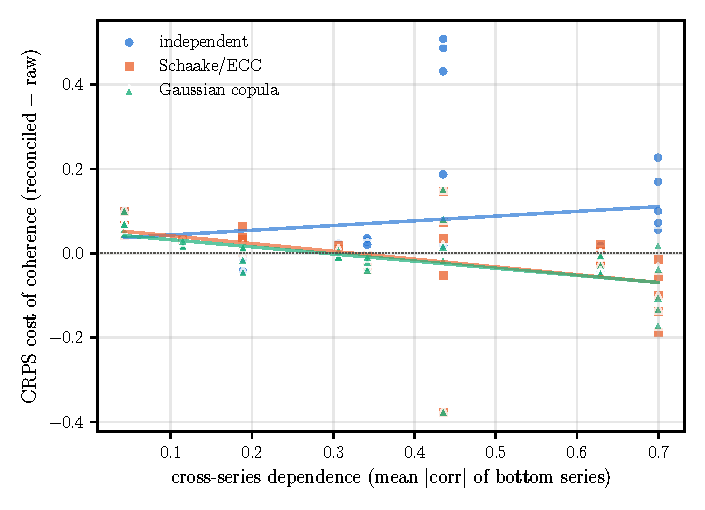
\includegraphics[width=\linewidth]{figures/prob_coherence_law.pdf}
\caption{CRPS cost of distributional coherence (reconciled $-$ raw) against
cross-series dependence, one point per foundation model and hierarchy ($40$ points,
eight hierarchies), for independent summation (circles), the Schaake shuffle
(squares) and the Gaussian copula (triangles). Lines are least-squares fits to the
plotted points; the statistics in the text are fitted across the eight hierarchies.}
\label{fig:probcohlaw}
\end{figure}

\subsection{Non-negativity}
\label{sec:nonneg}
The second constraint is per-series, and unlike coherence its treatment differs
sharply between models (Table~\ref{tab:nonneg}). On intermittent M5 retail series,
whose counts lie at zero, four of the five foundation models emit negative demand.
The severity varies widely. Moirai's median forecast is negative on $18.0\%$ of
series, Chronos-Bolt on $13.0\%$ and Chronos-2 on $0.9\%$, while TimesFM never does,
because its inference library by default guarantees a non-negative forecast when the
history is non-negative, a safeguard of the TimesFM~2.5 software rather than a property
described by \citet{timesfm2024}. Lower predictive bands are worse
still, negative on $67$--$72\%$ of series for every model except TimesFM.

Two observations qualify this. First, the violations appear where the data
approaches zero. On strictly positive M3 series, far from zero, every model is
nearly free of violations ($\le 0.02\%$ of medians, under $1\%$ of bands). The failure
is confined to the near-zero regime. Second, model
progress has addressed only half of it. Chronos-2 reduces negative medians more than
tenfold relative to Chronos-Bolt ($13.0\%\to 0.9\%$) yet improves the
negative lower band only marginally ($72.2\%\to 67.7\%$). A newer model therefore still
cannot be
deployed on non-negative data without an explicit projection. Non-negativity is
thus a deployment gap that some models close and others do not, and CAA closes it for
all by projection. None of them closes the coherence gap.


% AUTO-GENERATED by tsfm_bench.tables. Do not edit by hand.
\begin{table}[t]
\centering
\small
\begin{tabular}{lrrrr}
\toprule
& \multicolumn{2}{c}{M5 retail (near zero)} & \multicolumn{2}{c}{M3 (far from zero)} \\
\cmidrule(lr){2-3}\cmidrule(lr){4-5}
Model & median $<0$ & band $<0$ & median $<0$ & band $<0$ \\
\midrule
Moirai & 18.0 & 71.4 & 0.0 & 0.8 \\
C-Bolt & 13.0 & 72.2 & 0.0 & 0.3 \\
C-Bolt-B & 9.7 & 66.9 & 0.0 & 0.4 \\
C-2 & 0.9 & 67.7 & 0.0 & 0.3 \\
TimesFM & 0.0 & 0.0 & 0.0 & 0.0 \\
\bottomrule
\end{tabular}
\caption{Non-negativity violations: percentage of strictly non-negative series on which a zero-shot forecast goes below zero, for the median forecast and the lower ($10\%$) predictive band. Violations appear only where the data sits against the boundary (M5 retail counts), and are essentially absent far from it (M3). TTM = TinyTimeMixer; C-Bolt = Chronos-Bolt; C-Bolt-B = Chronos-Bolt-Base; C-2 = Chronos-2; LGBM = LightGBM.}
\label{tab:nonneg}
\end{table}


\subsection{Accuracy across foundation models}
\label{sec:frontier}
Finally we measure accuracy against per-series history length, an axis that most
foundation-model benchmarks do not vary and that only concurrent work has begun to
vary~\citep{breakeven2026,quitobench2026,energyload2026}, over three frequencies (M4
monthly
and quarterly, M5 daily), with eight rolling origins and $95\%$ bootstrap confidence
intervals (Table~\ref{tab:frontier}, Figure~\ref{fig:frontier}). With five foundation
models the heterogeneity among the models is larger than the effect being
measured. On smooth M4 data the best model changes repeatedly with history length:
a ten-parameter AutoETS is best at the shortest monthly history ($T=12$), Chronos-2 at
$T=48$ and $96$, TimesFM at $T=384$; and Moirai is worse than AutoETS at every
history length on both M4 datasets. The spread matters more than the ordering. At
$T=384$ the foundation models span $0.924$ (TimesFM) to $1.195$ (Moirai), and AutoETS,
at $0.993$, falls inside that interval. The spread among foundation models is
thus wider than the gap between them and the classical baseline, so the question
whether a foundation model is more accurate than a small one cannot be answered
without naming the foundation model.

The data regime matters as much as the model. On intermittent M5 series the picture
is different. All five foundation models outperform AutoETS at every history
length ($0.83$--$0.89$ against $1.03$--$1.08$) and cluster tightly, so there the
advantage is consistent and insensitive to model choice. We test every paired
comparison with a Wilcoxon signed-rank test and control the false discovery rate with
the Benjamini--Hochberg procedure. The $150$ comparisons set two small baselines
(AutoETS and CAA) against the five foundation models at each of the $15$
dataset\,$\times$\,history combinations, and $134$ remain significant at $q<0.05$.

This population-level verdict is not a per-series one. We also apply a
Diebold--Mariano test to each series individually, on the per-horizon loss differentials
and with the Harvey--Leybourne--Newbold small-sample correction that the per-series MASE
used above cannot support. It reaches a more conservative conclusion. On the smooth M4 data the ten-parameter AutoETS and the foundation models
are statistically indistinguishable on about $81\%$ of individual series, and above
$90\%$ for some model and history-length pairs. On intermittent M5 the foundation models are
significantly more accurate on $44$--$56\%$ of series, and the indistinguishable share
falls to $43$--$55\%$. The two
tests are not in conflict. With thousands of paired series a small mean difference is
readily detectable in aggregate, while on any given series the two forecasts
usually cannot be told apart. The practical reading is that the choice between a
foundation model and a ten-parameter alternative is, on smooth data, mostly
undetectable at the level at which forecasts are deployed. A study
evaluating one foundation model on one regime could therefore conclude either that
small models remain competitive or that they are obsolete, and both conclusions would
be defensible on their own evidence. The coherence results are not sensitive in this way. They hold
for every model, in the cross-sectional and in the temporal direction, whereas the
accuracy comparison does not hold across models.

The trained global baselines support this reading. On the two
energy hierarchies, where a model fit jointly across strongly correlated series might be
expected to be the most accurate, the covariate-free LightGBM and TCN are outperformed by the
leading foundation models. On Electricity the most accurate forecast is Chronos-2
($0.698$ MASE), against $0.99$ for the TCN and $1.12$ for LightGBM, and the ordering is
similar on Solar. This does not make foundation models categorically better. The
global baselines were given no exogenous covariates (calendar, weather), and with them
the ranking could differ; we do not test this. The accuracy result varies with the
data regime and the history length, whereas the coherence
failure, which these same global models show
(Section~\ref{sec:coherence}), varies with none of them.

\paragraph{CAA ablation}
Because CAA both selects a base and projects it, we isolate the two on a
capacity-constrained variant of M4-Monthly (a per-series ceiling). Conditioning the
selection on the declared capacity constraint changes the chosen base on $27\%$ of
series, but does not improve accuracy over a feature-only selection that is then
projected (mean MASE $0.864$ vs $0.875$; paired Wilcoxon $p=0.97$), while both are
exactly feasible because of the projection. Removing the projection instead allows
$9.9\%$ of forecast points to exceed the ceiling. The feasibility guarantee is thus a
property of the projection step, and we frame CAA accordingly.

% AUTO-GENERATED by tsfm_bench.tables. Do not edit by hand.
\begin{table}[t]
\centering
\small
\setlength{\tabcolsep}{4.5pt}
\begin{tabular}{lrrrrrr}
\toprule
$T$ & AutoETS & C-Bolt & C-Bolt-B & C-2 & Moirai & TimesFM \\
\midrule
\multicolumn{7}{l}{\emph{M4-Monthly}} \\
12 & \textbf{1.318} & 1.486 & 1.520 & 1.482 & 1.452 & 1.331 \\
48 & 1.084 & 1.137 & 1.124 & \textbf{1.028} & 1.307 & 1.041 \\
96 & 1.050 & 1.058 & 1.048 & \textbf{0.996} & 1.282 & 0.997 \\
384 & 0.993 & 1.008 & 1.010 & 0.973 & 1.195 & \textbf{0.924} \\
\midrule
\multicolumn{7}{l}{\emph{M4-Quarterly}} \\
8 & 1.561 & 1.593 & 1.593 & \textbf{1.436} & 2.096 & 1.590 \\
16 & \textbf{1.376} & 1.789 & 1.616 & 1.385 & 1.592 & 1.482 \\
128 & 1.277 & 1.357 & 1.309 & 1.262 & 1.406 & \textbf{1.233} \\
\midrule
\multicolumn{7}{l}{\emph{M5-daily}} \\
28 & 1.076 & 0.885 & 0.876 & 0.870 & 0.870 & \textbf{0.864} \\
224 & 1.029 & 0.850 & 0.851 & 0.841 & 0.844 & \textbf{0.835} \\
\bottomrule
\end{tabular}
\caption{Mean MASE against per-series history $T$ (best per row in bold), five foundation models and a ten-parameter AutoETS, over eight rolling origins. On the smooth M4 data the winner permutes with both $T$ and model choice and AutoETS lies inside the spread of the foundation models; on intermittent M5 every foundation model beats AutoETS decisively. Requiring eight origins restricts the sample to longer series, so these figures are not directly comparable with three-origin studies. TTM = TinyTimeMixer; C-Bolt = Chronos-Bolt; C-Bolt-B = Chronos-Bolt-Base; C-2 = Chronos-2; LGBM = LightGBM.}
\label{tab:frontier}
\end{table}


\begin{figure}[tbp]
\centering
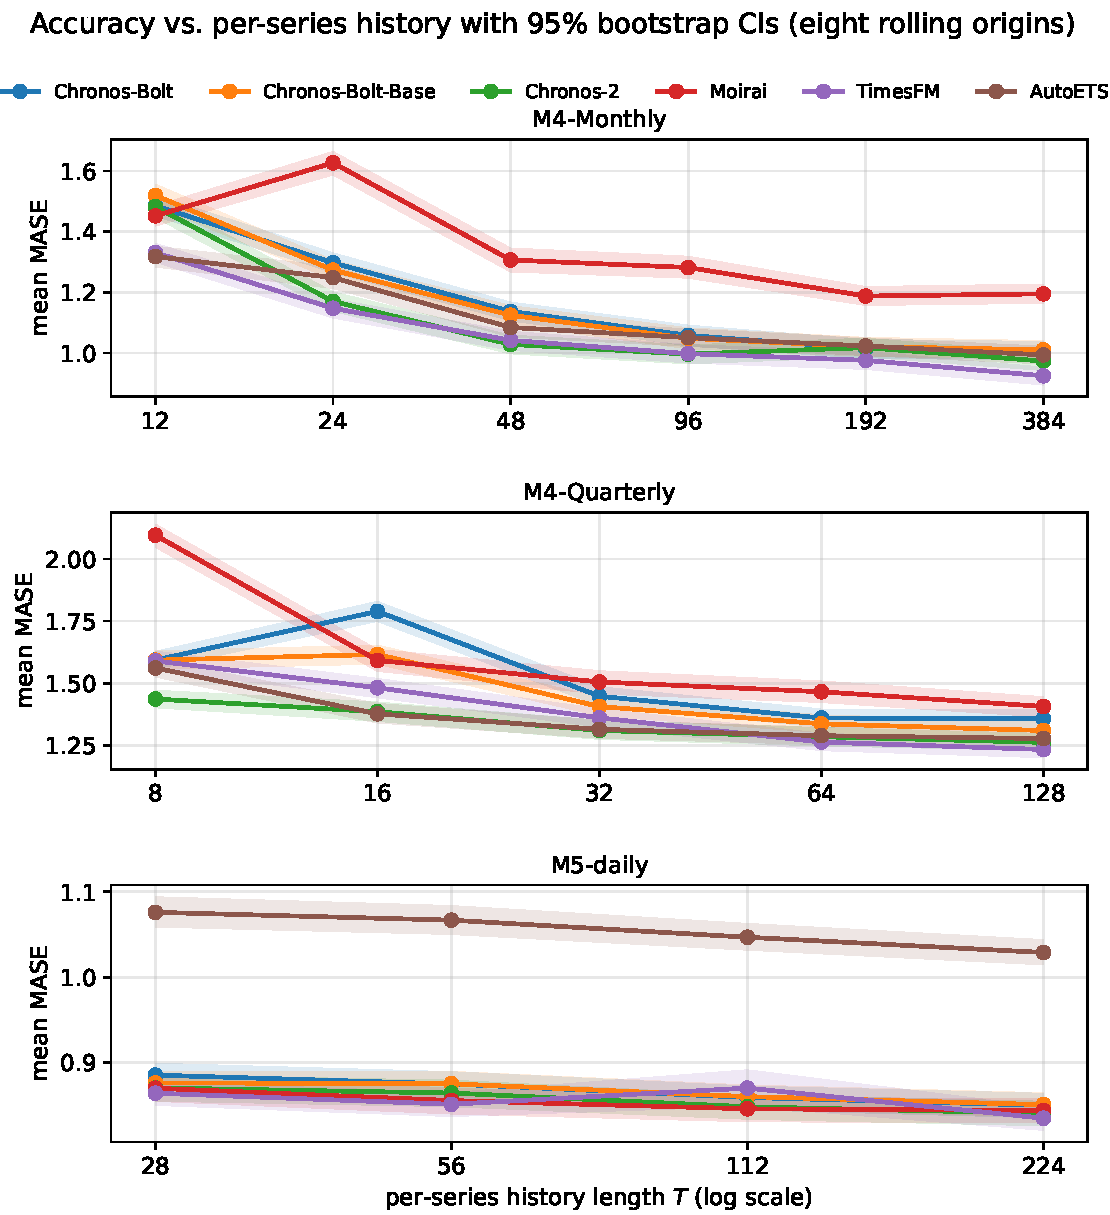
\includegraphics[width=\linewidth]{figures/frontier_study.pdf}
\caption{Mean MASE against per-series history length $T$, with $95\%$ bootstrap
confidence bands over eight rolling origins, for five foundation models and AutoETS.}
\label{fig:frontier}
\end{figure}

% ============================================================
\section{Discussion}
\label{sec:discussion}
A foundation model does not constrain its
outputs to satisfy a linear coupling relation among them, so it gives no guarantee of
satisfying one. On six of the eight real hierarchies the great majority of aggregate
nodes are incoherent for every foundation model but the least accurate, whose forecasts
are nearly flat. This includes
Chronos-2~\citep{chronos2_2025}, which accepts past and future covariates. Covariates condition each series' own forecast, but they do not couple
the forecasts across the hierarchy, so no amount of exogenous information restores
coherence. Chronos-2 and Moirai can also forecast several series
jointly~\citep{chronos2_2025,moirai2024}. We tested this mode for Chronos-2. It narrows
the gaps but leaves most aggregates incoherent on five of the eight hierarchies
(Section~\ref{sec:coherence}), because sharing information across series is not a
constraint on their sum. We did not evaluate Moirai's joint mode. The
same failure
appears between the temporal aggregations of a single series, where the coupling
involves no second series. This removes the objection that the hierarchy should
have been modelled jointly.

Nor is the failure a property of per-series modelling specifically. Two trained global
models, fit jointly across every series of a hierarchy, are incoherent at comparable
rates (Section~\ref{sec:coherence}), so the failure belongs to any forecaster whose
outputs are not projected onto the coupling set. It does
not depend on which model is used or on its accuracy. It is therefore a property of
unconstrained forecasting, and we do not claim it
as a defect peculiar to foundation models. It matters for them because of the way they
are deployed. They are offered as general-purpose forecasters that require no
per-series modelling, they are assessed by benchmarks that do not measure
coherence~\citep{gifteval2024,fevbench2025}, the agentic systems proposed around
forecasting do not enforce it~\citep{tsci2025,nexus2026,dcats2025}, and they are used by
analysts who
cannot refit them. The two supporting results do not share this stability. Per-series accuracy is sufficiently heterogeneous
that a ten-parameter classical model outperforms Moirai at every history length on the
smooth M4 data yet is less accurate than TimesFM at most of them, and
non-negativity is enforced by one model and not the others. Each of these verdicts
depends on which model is used; the coherence result does not. A
forecasting system for hierarchical or otherwise constrained data should therefore not
treat a foundation model as a complete solution. It requires an explicit
reconciliation or projection step, applied to whichever base is most accurate,
whether a reconciled foundation model or a small interpretable one. CAA supplies that
step by construction.

The probabilistic case is more demanding. For point forecasts the reconciliation step
costs little accuracy and takes a fraction of a second (Table~\ref{tab:timing}), and
even for the predictive distributions these models also emit, summing independent
marginals is usually inexpensive. Summing independent marginals, however, discards the
cross-series dependence, which a per-series model never supplies. A copula must
reconstruct that joint from
history and can only approximate it. Coherence of the distribution is attainable by
construction; the true joint, and hence a calibrated aggregate distribution, is not
recoverable from the model's own marginals.

\paragraph{Limitations} The coherence finding is well supported by eight hierarchies,
six foundation models plus two trained global baselines, and point-reconciliation
accuracy over up to eight rolling origins with bootstrap confidence intervals. Point
reconciliation uses bottom-up. We found MinTrace-OLS unstable on Wiki2 and rarely better
than bottom-up elsewhere: in $6$ of the $64$ combinations of eight base models (the six
foundation models and the two global ones) with eight hierarchies, by at most $0.05$
MASE. Its shrinkage variant, run on the six foundation models, was stable everywhere but
better than bottom-up in only $21$ of $48$ combinations. The learned ERM
reconciler~\citep{bentaieb2019erm} was stable on only one of eight hierarchies, its
reconciliation matrix under-determined from the small number of in-sample origins we
allow every base. A learned
reconciler with more in-sample signal, or a score-optimal probabilistic one, is a natural
extension but was not the reliable choice here. On the probabilistic side, we deliberately
enlarged the sample with two high-dependence hierarchies (Electricity, Solar) to test
whether the independent-summation cost scales with cross-series dependence. It does not,
so we report the coupling benefit, which does hold. Traffic is
the one costly case, and a tighter characterisation of when independent summation is
costly remains open.
The accuracy-heterogeneity comparison uses paired
Wilcoxon signed-rank tests with Benjamini--Hochberg false-discovery control,
complemented by per-series Diebold--Mariano tests on per-horizon losses. We compute the
latter on a subsample ($178$--$392$ series per dataset after filtering) rather than the
full panel.

\section{Conclusions}
\label{sec:conclusions}
Time-series foundation models forecast each series on its own and apply no constraint
across their outputs, so the forecasts for the parts of a hierarchy need not add up to
the forecast for the whole. This paper measured how often six such models, used
zero-shot, violate coupling constraints of this kind and what it costs to restore them. On six of the eight hierarchies most aggregate nodes are
incoherent for five of the six foundation models. The sixth, the least accurate, falls
below half on two of them, where its forecasts are nearly flat. The rates do not
otherwise vary with accuracy or with model size. A classical model and two global models trained jointly
across the hierarchy are incoherent at comparable rates, and Chronos-2, run in its joint
mode, reduces the gaps without closing them. The same failure appears within a single
series, where each model contradicts itself on between roughly a third and four fifths
of its own temporal aggregates. The failure is therefore a property of unconstrained
forecasting, and it matters for foundation models because they are deployed without a
step that would constrain them.

For point forecasts the failure is removed at low cost. Bottom-up reconciliation restores
coherence with a small loss of accuracy, more reliably than the OLS form of trace
minimisation or a learned reconciler, and in the temporal case it improves accuracy. On
all eight hierarchies the most accurate coherent forecast is a reconciled foundation
model. For predictive distributions the failure is only partly removed. Summing
independent marginals is coherent by construction and usually inexpensive, and its cost
does not grow with cross-series dependence. The marginals, however, omit the joint
distribution, which a copula fitted to history can only approximate. An accurate
coherent predictive distribution from a per-series base therefore remains open.

The two supporting results behave differently from coherence. Per-series accuracy varies
more across the foundation models than between them and a ten-parameter classical model,
so it does not identify a best base. Non-negativity is satisfied by one model and
violated by the others. Of the three constraints audited, only coherence is violated by
every model.

For a forecasting system that uses these models on constrained data, the results imply
that a foundation model supplies a base forecast and that the system has to add an
explicit reconciliation or projection step, applied to whichever base is most accurate.
The audit does not identify that base in advance. Constraint-aware
assembly adds that step for a small interpretable base, and the ablation attributes its
feasibility guarantee to the projection step alone. When the model selection is
conditioned on the declared constraints, the chosen base changes but accuracy and
feasibility do not, so the guarantee does not depend on how the base is chosen.

% ============================================================
\section*{Declaration of generative AI and AI-assisted technologies in the manuscript preparation process}
During the preparation of this work the authors used Claude Code (Anthropic) in
order to assist with code scaffolding for the experiments, to translate into English
portions of the manuscript originally written in Spanish, and for language editing.
After using this tool/service, the authors reviewed and edited
the content as needed and take full responsibility for the content of the
publication.

\section*{Declaration of competing interest}
The authors declare that they have no known competing financial interests or
personal relationships that could have appeared to influence the work reported in
this paper.

\section*{CRediT authorship contribution statement}
\textbf{Lino González García:} Conceptualization, Methodology, Software,
Investigation, Writing -- original draft, Writing -- review \& editing.
\textbf{Loukas Samaras:} Investigation, Methodology, Validation, Writing -- review \&
editing. \textbf{Elena García-Barriocanal:} Conceptualization, Methodology,
Investigation, Validation, Writing -- review \& editing. \textbf{Miguel-Angel
Sicilia:} Conceptualization, Methodology, Investigation, Validation, Supervision,
Writing -- review \& editing.

\section*{Funding}
This research did not receive any specific grant from funding agencies in the public,
commercial, or not-for-profit sectors.

\section*{Data availability}
All datasets used in this study are publicly available and no new data were generated.
The M3~\citep{data_m3}, M4~\citep{data_m4} and M5~\citep{data_m5} forecasting
competition data and the five benchmark hierarchies (TourismSmall and
TourismLarge~\citep{data_tourism,hyndman2011,mint2019}, Labour, and the Traffic and Wiki2
hierarchies of \citet{bentaieb2019erm}) are accessed
through the open
\texttt{datasetsforecast} package~\citep{datasetsforecast}. The Solar and Electricity hierarchies are constructed
from the hourly \texttt{solar\_nips} and \texttt{electricity\_nips} collections used
by \citet{salinas2019gpcopula} and distributed with GluonTS~\citep{gluonts2020}, the
latter derived from \citet{data_electricity}.

The code that downloads every dataset, builds the hierarchies and reproduces every
experiment, table and figure in this paper is publicly available at
\url{https://github.com/msicilia/tsfm-coherence-audit}.

% Neurocomputing: numbered references in order of appearance; the -names variant
% lets \citet print "Author et al. [n]" as the guide for authors shows.
\bibliographystyle{elsarticle-num-names}
\bibliography{references}

\end{document}
